% Set up the standalone document class
\documentclass{standalone}

% Input the preamble (<3)
% Preamble document

% Import tikz package
\usepackage{tikz}

% Import tikz libraries
\usetikzlibrary{shapes, arrows}
\usetikzlibrary{positioning, calc}

%----------- Create a fancy summing block
\tikzset{add/.style n args={4}{
		minimum width=6mm,
		path picture={
			\draw[black] 
			(path picture bounding box.south east) -- (path picture bounding box.north west)
			(path picture bounding box.south west) -- (path picture bounding box.north east);
			\node at ($(path picture bounding box.south)+(0,0.13)$)     {\tiny #1};
			\node at ($(path picture bounding box.west)+(0.13,0)$)      {\tiny #2};
			\node at ($(path picture bounding box.north)+(0,-0.13)$)    {\tiny #3};
			\node at ($(path picture bounding box.east)+(-0.13,0)$)     {\tiny #4};
		}
	}
}

%----------- Block style 1
\tikzstyle{block1} = [draw, fill=blue!20, rectangle, 
minimum height=3em, minimum width=6em, node distance=2.5cm]

%----------- Block style 2
\tikzstyle{block2} = [draw, fill=blue!20, rectangle, 
minimum height=3em, minimum width=3em, node distance=2.5cm]

%----------- Sum style
\tikzstyle{sum} = [draw, fill=blue!20, circle, node distance=2cm]

%----------- Input style
\tikzstyle{input} = [coordinate, node distance=4cm]

%----------- Output style
\tikzstyle{output} = [coordinate, node distance=4cm]

%----------- Pin style
\tikzstyle{pinstyle} = [pin edge={to-,thin,black}]

\usetikzlibrary{positioning}

\tikzset{basic/.style={draw,fill=blue!20,text width=1em,text badly centered}}
\tikzset{input/.style={basic,circle}}
\tikzset{weights/.style={basic,rectangle}}
\tikzset{functions/.style={basic,circle,fill=blue!10}}

\begin{document}

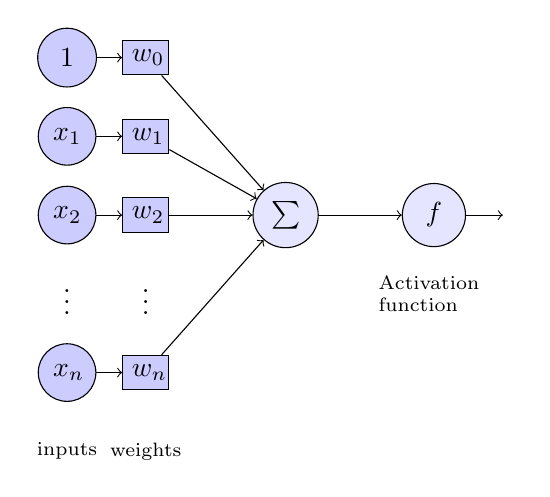
\begin{tikzpicture}
   	\node[functions] (center) {$f$};
	\node[below of=center,font=\scriptsize,text width=4em] {Activation function};
	%\draw[thick] (0.5em,0.5em) -- (0,0.5em) -- (0,-0.5em) -- (-0.5em,-0.5em);
	%\draw (0em,0.75em) -- (0em,-0.75em);
	%\draw (0.75em,0em) -- (-0.75em,0em);
	\node[right of=center] (right) {};
    	\path[draw,->] (center) -- (right);
	\node[functions,left=3em of center] (left) {$\sum$};
    	\path[draw,->] (left) -- (center);
	\node[weights,left=3em of left] (2) {$w_2$} -- (2) node[input,left of=2] (l2) {$x_2$};
    	\path[draw,->] (l2) -- (2);
    	\path[draw,->] (2) -- (left);
	\node[below of=2] (dots) {$\vdots$} -- (dots) node[left of=dots] (ldots) {$\vdots$};
	\node[weights,below of=dots] (n) {$w_n$} -- (n) node[input,left of=n] (ln) {$x_n$};
    	\path[draw,->] (ln) -- (n);
    	\path[draw,->] (n) -- (left);
	\node[weights,above of=2] (1) {$w_1$} -- (1) node[input,left of=1] (l1) {$x_1$};
    	\path[draw,->] (l1) -- (1);
    	\path[draw,->] (1) -- (left);
	\node[weights,above of=1] (0) {$w_0$} -- (0) node[input,left of=0] (l0) {$1$};
    	\path[draw,->] (l0) -- (0);
    	\path[draw,->] (0) -- (left);
	\node[below of=ln,font=\scriptsize] {inputs};
	\node[below of=n,font=\scriptsize] {weights};
\end{tikzpicture}

\end{document}